\section*{\underline{PART E: Statistical Inference}}
\markboth{PART E: Statistical Inference}{}

\subsection*{Question 11: Is there sufficient statistical evidence that the true mean repair time exceeds the company's 15-minute target?}

\textit{Note: The original management target of 60 minutes was adjusted to a 15-minute target for this analysis to better align with the reality of the observed dataset.}

To determine if the true average repair time significantly exceeds the 15-minute target, we conducted a one-sample right-tailed t-test. The hypotheses are defined as:


\begin{center}
    \fbox{
        \begin{minipage}{0.65\textwidth}
            \centering
            \textbf{Hypotheses}

            \vspace{0.15cm}

            \textbf{Null Hypothesis:} $\mu = 15$ minutes

            \vspace{0.1cm}

            \textbf{Alternative Hypothesis:} $\mu > 15$ minutes

            \vspace{0.1cm}
        \end{minipage}
    }
\end{center}



Using the baseline dataset, the hypothesis test yielded the following results:
\begin{itemize}
    \item \textbf{Target Mean:} 15.00 minutes
    \item \textbf{Sample Mean:} 16.36 minutes
    \item \textbf{Sample Size ($n$):} 635
    \item \textbf{T-Statistic:} 1.5433
    \item \textbf{P-Value:} 0.0616
    \item \textbf{Significance Level ($\alpha$):} 0.05
\end{itemize}



This relationship is visualized in Figure \ref{fig:ttest_target}, showing the target mean versus our sample mean along the theoretical sampling distribution.

\begin{figure}[H]
    \centering
    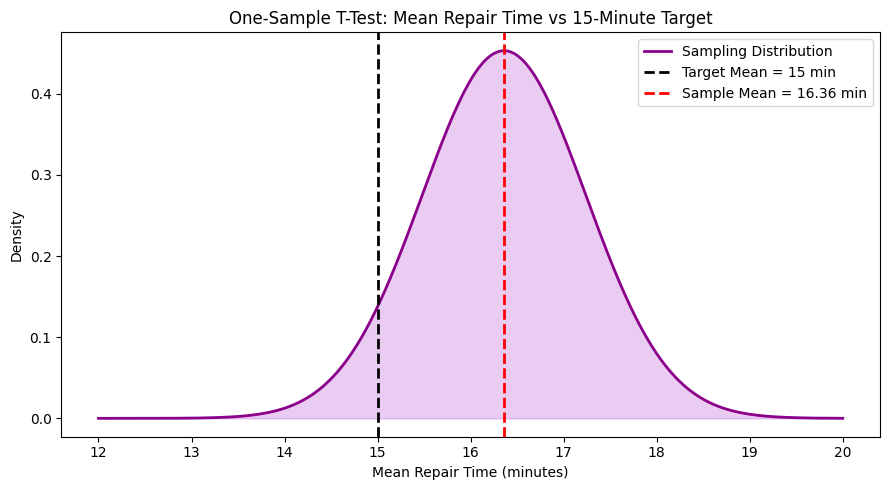
\includegraphics[width=0.85\linewidth]{figures/target.png}
    \caption{One-Sample T-Test: Sampling distribution comparing the 15-minute target mean against the observed sample mean of 16.36 minutes.}
    \label{fig:ttest_target}
\end{figure}

\textbf{Conclusion:} Because our calculated p-value (0.0616) is greater than the significance level ($\alpha = 0.05$), we \textbf{fail to reject the null hypothesis}. Although the sample mean of 16.36 minutes is mathematically higher than 15 minutes, this difference is not statistically significant. There is insufficient statistical evidence to conclude that the true plant-wide population mean repair time exceeds the 15-minute target. 

Furthermore, supporting this baseline performance, our probability estimation indicates that there is a \textbf{65.02\% probability} that any random repair event will be successfully completed in less than the 15-minute target time.

\subsection*{Question 12: Is the mean repair time different between morning and afternoon shifts?}

\textit{Note: Based on the operational timestamps available in the dataset, the analysis was adapted to compare Morning and Afternoon shifts rather than day and night shifts.}

To determine if the time of day impacts maintenance efficiency, we conducted an independent two-sample t-test (assuming unequal variances) to compare the mean repair times between the morning and afternoon production shifts. The hypotheses are defined as:
% \begin{itemize}
%     \item \textbf{Null Hypothesis ($H_0$):} $\mu_{\text{morning}} = \mu_{\text{afternoon}}$ (There is no difference in mean repair times)
%     \item \textbf{Alternative Hypothesis ($H_A$):} $\mu_{\text{morning}} \neq \mu_{\text{afternoon}}$ (There is a difference in mean repair times)
% \end{itemize}


\begin{center}
    \fbox{
        \begin{minipage}{0.98\textwidth}
            \centering
            \textbf{Hypotheses}

            \vspace{0.15cm}

            \textbf{Null Hypothesis:}
            $\mu_{\text{morning}} = \mu_{\text{afternoon}}$ (There is no difference in mean repair times)

            \vspace{0.1cm}

            \textbf{Alternative Hypothesis:}
            $\mu_{\text{morning}} \neq \mu_{\text{afternoon}}$ (There is a difference in mean repair times)

            \vspace{0.1cm}
        \end{minipage}
    }
\end{center}


The results of the hypothesis test are summarized below:
\begin{itemize}
    \item \textbf{Morning Shift Mean:} 14.45 minutes 
    \item \textbf{Morning Repairs ($n_1$):} 387
    \item \textbf{Afternoon Shift Mean:} 19.34 minutes 
    \item \textbf{Afternoon Repairs ($n_2$):} 248
    \item \textbf{T-Statistic:} -2.8088
    \item \textbf{P-Value:} 0.0051
\end{itemize}

\textbf{Conclusion:} Because the calculated p-value (0.0051) is well below the standard 0.05 significance level, we \textbf{reject the null hypothesis}. There is strong, statistically significant evidence indicating a difference in mean repair times between the two shifts. Specifically, repairs conducted during the afternoon shift take significantly longer on average (by nearly 5 minutes) compared to those completed in the morning.

Figure \ref{fig:shift_comparison} visualizes this disparity, displaying the distinct distributions and the upward shift in the mean during the afternoon operational hours.

\begin{figure}[H]
    \centering
    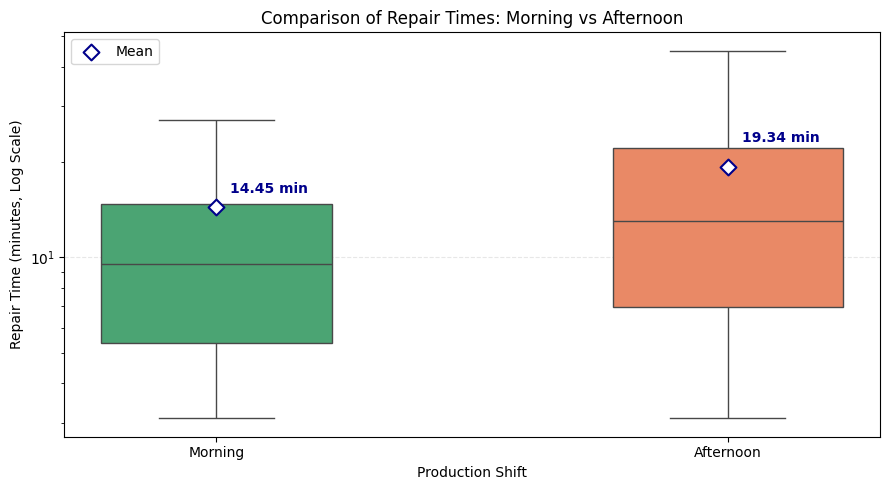
\includegraphics[width=0.85\linewidth]{figures/shift-day-night.png}
    \caption{Comparison of Repair Times between Morning and Afternoon Shifts (Log Scale). The diamond markers indicate the sample means for each shift.}
    \label{fig:shift_comparison}
\end{figure}

\subsection*{Question 13: Did the new maintenance procedure reduce repair time?}

To address this question, we must first define the ``new maintenance procedure.'' For this facility, management implemented a Lean Six Sigma (LSS) framework. Lean Six Sigma is a hybrid process-improvement methodology: ``Lean'' focuses on eliminating waste and unnecessary steps to increase operational speed, while ``Six Sigma'' relies on statistical data to reduce process variation and eliminate defects. 

To evaluate whether this new LSS procedure was successful, we conducted a two-sample t-test comparing the repair times from our baseline dataset (\texttt{DowntimeDataset.csv}) against the repair times recorded post-LSS implementation (\texttt{DowntimeDataset\_afterLSS.csv}).

The hypotheses are defined as:

\begin{center}
    \fbox{
        \begin{minipage}{0.95\textwidth}
            \centering
            \textbf{Hypotheses}

            \vspace{0.15cm}

            \textbf{Null Hypothesis:}
            $\mu_{\text{Before LSS}} = \mu_{\text{After LSS}}$ (The new procedure did not reduce mean repair time)

            \vspace{0.15cm}

            \textbf{Alternative Hypothesis:}
            $\mu_{\text{Before LSS}} > \mu_{\text{After LSS}}$ (The new procedure significantly reduced mean repair time)

            \vspace{0.1cm}
        \end{minipage}
    }
\end{center}


The results of the hypothesis test are summarized below:
\begin{itemize}
    \item \textbf{Mean Repair Time (Before LSS):} 16.36 minutes ($n_1 = 635$)
    \item \textbf{Mean Repair Time (After LSS):} 16.13 minutes ($n_2 = 540$)
    \item \textbf{T-Statistic:} 0.1321
    \item \textbf{P-Value:} 0.4475
\end{itemize}

\textbf{Conclusion:} Because the calculated p-value (0.4475) is overwhelmingly larger than the standard significance level ($\alpha = 0.05$), we \textbf{fail to reject the null hypothesis}. While there was a nominal decrease in the average repair time (from 16.36 to 16.13 minutes), this difference of roughly 14 seconds is merely mathematical and not statistically significant. There is insufficient statistical evidence to conclude that the Lean Six Sigma implementation successfully reduced the mean machine repair time.

Figure \ref{fig:lss_impact} illustrates this finding, showing that the probability density distributions and the sample means for both periods are almost entirely overlapping.

\begin{figure}[H]
    \centering
    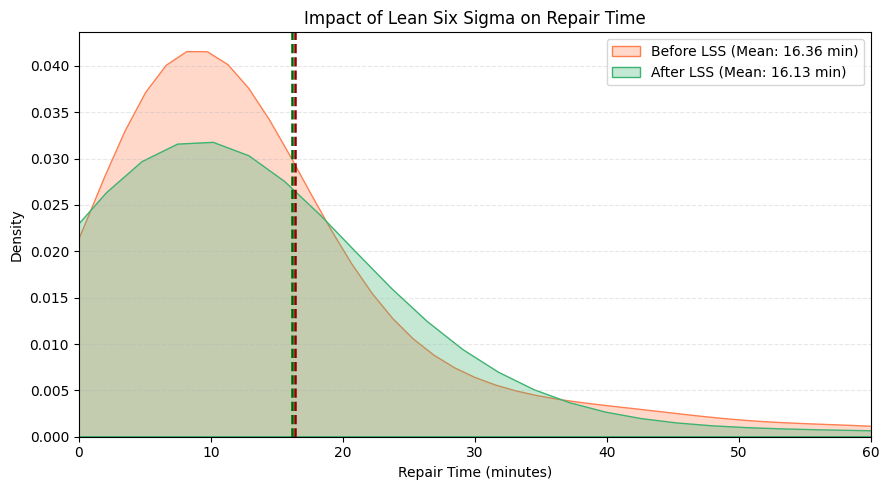
\includegraphics[width=0.85\linewidth]{figures/LSS-repair_time.png}
    \caption{Impact of Lean Six Sigma on Repair Time. The distributions before and after LSS implementation show near-identical means, indicating no statistically significant reduction in downtime.}
    \label{fig:lss_impact}
\end{figure}

\subsection*{Question 14: Does mean repair time differ among different failure groups?}

\textit{Note: As established in our contextual assumptions, the raw dataset does not record explicit ``failure severity'' levels (Low, Medium, High). Instead, we utilized the broad stoppage categories (\texttt{StopGroup})—FAILURE, MATERIALS, and OPERATIONAL—as a proxy for the type and complexity of the downtime event to answer this question.}

To determine if the downtime category significantly impacts the length of the stoppage, we conducted a One-Way Analysis of Variance (ANOVA). The hypotheses are defined as:

\begin{center}
    \fbox{
        \begin{minipage}{0.95\textwidth}
            \centering
            \textbf{Hypotheses}

            \vspace{0.15cm}

            \textbf{Null Hypothesis:}
            $\mu_{\text{FAILURE}} = \mu_{\text{MATERIALS}} = \mu_{\text{OPERATIONAL}}$
            (All categories have the same mean repair time)

            \vspace{0.15cm}

            \textbf{Alternative Hypothesis:}
            At least one category has a significantly different mean repair time.

            \vspace{0.1cm}
        \end{minipage}
    }
\end{center}

\vspace{1cm}

The ANOVA test results are detailed below:
\begin{itemize}
    \item \textbf{FAILURE:} Mean = 14.57 minutes ($n = 222$)
    \item \textbf{MATERIALS:} Mean = 12.54 minutes ($n = 189$)
    \item \textbf{OPERATIONAL:} Mean = 24.64 minutes ($n = 127$)
    \item \textbf{F-Statistic:} 11.9403
    \item \textbf{P-Value:} $8.45 \times 10^{-6}$ (or 0.00000845)
\end{itemize}

\textbf{Conclusion:} Because the calculated p-value is extremely small and well below our significance level ($\alpha = 0.05$), we \textbf{reject the null hypothesis}. There is strong, statistically significant evidence indicating a difference in mean repair times among the groups. Specifically, \texttt{OPERATIONAL} stoppages take substantially longer to resolve (an average of 24.64 minutes) compared to direct mechanical \texttt{FAILURE} events (14.57 min) or \texttt{MATERIALS}-related delays (12.54 min).

Figure \ref{fig:failure_type} displays the distribution of repair times across these three groups using violin plots, clearly highlighting the upward shift in the operational delays category.

\begin{figure}[H]
    \centering
    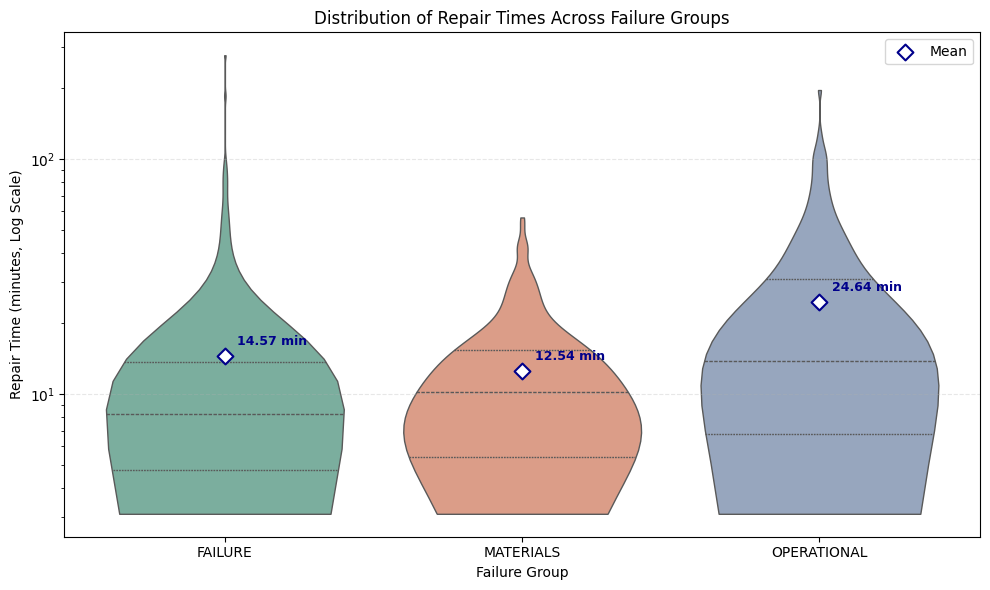
\includegraphics[width=0.85\linewidth]{figures/failure-type.png}
    \caption{Distribution of Repair Times Across Failure Groups (Log Scale). The diamond markers denote the distinct mean durations for each stoppage category.}
    \label{fig:failure_type}
\end{figure}


\subsection*{Question 15: Is the variability in repair time acceptable?}

To evaluate whether the variability in machine repair times is within the
company's acceptable limit, we conducted a Chi-Square test for a single
population variance. For this analysis, only repair records belonging to
the MATERIALS category were considered. The company's acceptable upper
limit for the standard deviation was set at 10.00 minutes, corresponding
to a maximum acceptable variance of 100.00 $\text{min}^2$.

\vspace{2cm}
The hypotheses for this right-tailed test are defined as:

\begin{center}
    \fbox{
        \begin{minipage}{0.95\textwidth}
            \centering
            \textbf{Hypotheses}

            \vspace{0.15cm}

            \textbf{Null Hypothesis:}
            $\sigma^2 = 100$
            (The population variance is within the acceptable limit)

            \vspace{0.15cm}

            \textbf{Alternative Hypothesis:}
            $\sigma^2 > 100$
            (The population variance exceeds the acceptable limit)

            \vspace{0.1cm}
        \end{minipage}
    }
\end{center}

The results of the Chi-Square test are summarized below:

\begin{itemize}
    \item \textbf{Acceptable Variance Target:}
    100.00 $\text{min}^2$ (SD = 10.00 min)

    \item \textbf{Sample Variance:}
    93.22 $\text{min}^2$ (SD = 9.66 min)

    \item \textbf{Sample Size ($n$):} 189

    \item \textbf{Chi-Square Statistic:} 175.2613

    \item \textbf{P-Value:} 0.738203
\end{itemize}

\textbf{Conclusion:}
Since the calculated p-value (0.738203) is greater than the
significance level of 0.05, we fail to reject the null hypothesis.
There is insufficient statistical evidence to conclude that the
population variance of repair times in the MATERIALS category exceeds
the company's acceptable limit.

The observed sample standard deviation is 9.66 minutes, which is
slightly below the acceptable limit of 10.00 minutes. Thus, the
observed variability is within the specified target, although the
hypothesis test does not establish that the population variance
definitively satisfies the requirement.

Figure \ref{fig:variance_target} compares the actual repair-time
distribution for the MATERIALS category with the acceptable target
distribution.

\begin{figure}[H]
    \centering
    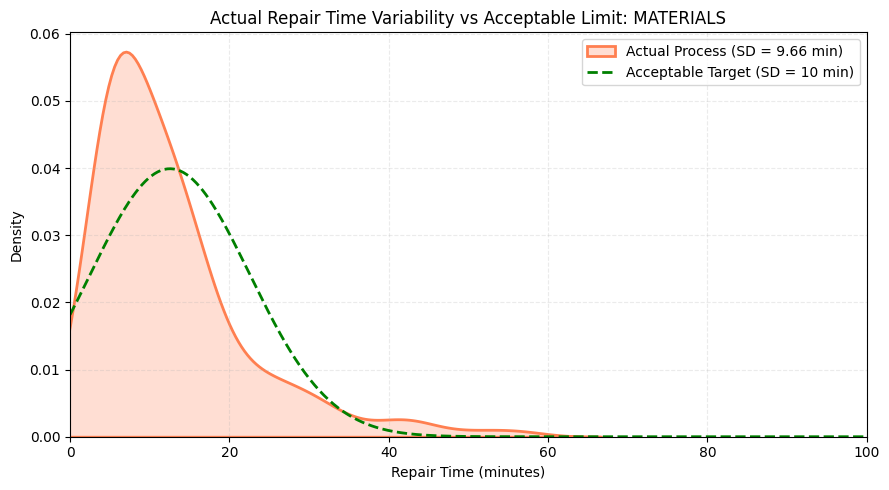
\includegraphics[width=0.85\linewidth]{figures/variance-target.png}
    \caption{Actual Repair Time Variability vs Acceptable Limit for
    the MATERIALS category. The actual process distribution
    (solid orange) has a sample standard deviation of 9.66 minutes,
    compared with the acceptable target distribution
    (dashed green) with a standard deviation of 10 minutes.}
    \label{fig:variance_target}
\end{figure}


\subsection*{Question 16: Proportion of Repairs Exceeding a Specified Duration}

The objective is to determine whether the proportion of repairs exceeding a specified
duration is greater than the acceptable limit of 10\%. To examine how the choice of
duration threshold affects the result, three thresholds (25, 30, and 35 minutes) are
considered.

A one-sample exact binomial test is performed for each threshold. Let $p$ denote the
population proportion of repairs exceeding the specified duration.

\begin{center}
    \fbox{
        \begin{minipage}{0.65\textwidth}
            \centering
            \textbf{Hypotheses}

            \vspace{0.15cm}

            \textbf{Null Hypothesis:} $p = 0.10$

            \vspace{0.1cm}

            \textbf{Alternative Hypothesis:} $p > 0.10$

            \vspace{0.1cm}
        \end{minipage}
    }
\end{center}

The significance level is set to $\alpha = 0.05$. The test results are summarized below.

\begin{table}[htbp]
    \centering
    \caption{Binomial test results for different repair-duration thresholds}
    \label{tab:q16_binomial}
    \begin{tabular}{|c|c|c|c|}
        \hline
        \textbf{Duration Threshold} &
        \textbf{Observed Proportion} &
        \textbf{p-value} &
        \textbf{Decision} \\
        \hline
        25 minutes & 14.33\% & 0.000341 & Reject $H_0$ \\
        \hline
        30 minutes & 11.18\% & 0.176499 & Fail to reject $H_0$ \\
        \hline
        35 minutes & 8.98\% & 0.822189 & Fail to reject $H_0$ \\
        \hline
    \end{tabular}
\end{table}

\textbf{Interpretation:}

At the 25-minute threshold, the p-value (0.000341) is below the significance level
of 0.05. Therefore, the null hypothesis is rejected. There is sufficient statistical
evidence that more than 10\% of repairs take longer than 25 minutes.

For the 30-minute and 35-minute thresholds, the p-values are greater than 0.05.
Hence, the null hypothesis cannot be rejected for either threshold. There is
insufficient statistical evidence to conclude that more than 10\% of repairs exceed
these durations.

\textbf{Conclusion and Engineering Implication:}
The proportion of repairs exceeding 25 minutes is significantly greater than the acceptable limit of 10\%, while no significant evidence is found at the 30- and 35-minute thresholds. Therefore, repairs exceeding 25 minutes deserve further investigation to identify potential delays. The 10\% benchmark is assumed and should be validated against operational requirements. These results represent a threshold-based sensitivity analysis using the same dataset.